\documentclass{article}

\usepackage{enumerate}
\usepackage{amsmath,amsthm,amssymb}
\usepackage{tikz}
\usepackage{pgfplots}
\usepackage{multicol}
%\pgfplotsset{compat=newest}

\usepackage[margin=1in]{geometry}

\begin{document}

\noindent \textbf{Name:}\underline{\hspace{2in}} \hfill \textbf{Quadratic Optimization Re-Take}
\\ \\
Class time (circle one): 9:30 am \hspace{1cm} 11:00am
\vspace{1em}

The cost of producing $q$ items is $C(q) = 0.37 q + 10$. When $q$ items are produced, they will be sold for a price of $P(q) = 16 - 1.5 q$. Profit is revenus minus costs, i.e.,
  \[
    \text{Profit}(q) = q \cdot P(q) - C(q).
  \]

  \begin{enumerate}
  \item (3 points) Write an equation for $\text{Profit}(q)$, only in terms of $q$. Simplify your answer completely.
    \vspace{2.5in}
  \item (5 points) Sketch a graph of $\text{Profit}(q)$, and identify which kind of function it is. Remember to label your axes!
    \begin{multicols}{2}
      % \includegraphics[scale=0.7]{axes.png}
      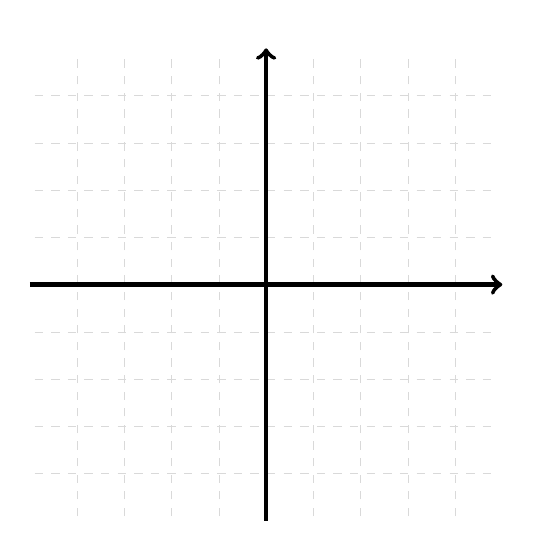
\begin{tikzpicture}[scale=0.6]
\draw[help lines, color=gray!30, dashed] (-4.9,-4.9) grid (4.9,4.9);
\draw[->,ultra thick] (-5,0)--(5,0) node[right]{};
\draw[->,ultra thick] (0,-5)--(0,5) node[above]{};
\end{tikzpicture}
      \columnbreak
      ~\\
        $\operatorname{Profit}(q)$ is a \underline{\hspace{8em}} function:
        \begin{enumerate}[(a)]
          \setlength\itemsep{2.5em}
          \item Linear
          \item Quadratic
          \item Greatest integer
          \item Always Increasing
          \item Always Decreasing
        \end{enumerate}
    \end{multicols}
\pagebreak
\item (4 points) Does $\text{Profit}(q)$ have a minimum value, maximum value, or neither? Find the extreme value, or explain why no such value exists.
  \vspace{3in}
\item (3 points) Interpret your answer to Question 3. Does your answer make sense? Explain why or why not.
  
\end{enumerate}

\end{document}
